In this section,
the effects of applying repetition learning on the performance of the proposed method and the important role of the task embedding network $E$ are discussed in detail.


The experimental results assessed in the previous section have shown the potential of the proposed adaptation method in tackling the task adaptation problem in imitation learning.
As shown in Tables \ref{ch:DTAIL:tab:Result_SuccessRate_Before_Source} and \ref{ch:DTAIL:tab:Result_SuccessRate_After_Target},
the proposed method could provide consistent and high performance in terms of success rate and average cumulative reward on both source and target tasks with varying difficulty levels.
This indicates that the proposed method can be applied to more challenging tasks with larger state and action spaces.
Moreover,
Table \ref{ch:DTAIL:tab:Result_SuccessRate_After_Source} shows that the performance deterioration on the source task was also reduced compared to transfer learning baselines.
This promising result demonstrates the effectiveness of the proposed adaptation method,
in which the idea of repetition learning was leveraged in order to allow the agent to review the previously learned source task.
Although the success rate and training time remained limited,
the proposed method presents a plausible approach to tackle the task adaptation problem in imitation learning.
It can be further improved in order to provide better overall performance toward practical imitation learning tasks.



In order to support the idea of repetition learning,
an imitation learning agent was proposed, which was able to encode its learned knowledge into a task-embedding space.
To provide an ablation study of the task embedding network $E$ in the proposed agent,
a small experiment was conducted, where a number of task embeddings $z^t_S$ and $z^t_T$ were collected by executing the adapted agent in the WindowOpen--WindowClose experiment on both source task (i.e., WindowOpen) and target task (i.e., WindowClose).
The WindowOpen--WindowClose was chosen because both source and target tasks are similar and have a large and equal size of the state space, which can provide a sufficient ablation result.
In each task,
the adapted agent was run in the simulation over 100 trials.
After that,
t-distributed stochastic neighbor embedding (t-SNE) was applied in order to project the collected high-dimensional task embeddings to a two-dimensional space for visualization as shown in Figure \ref{ch:DTAIL:fig:TSNE}.
t-SNE captures the distance relation between task embeddings.
If two embeddings were close in the task-embedding space,
they stay close in the resulting visualization,
and vice versa.
Therefore,
from Figure \ref{ch:DTAIL:fig:TSNE},
it can be seen that task embeddings of the source and target tasks were well separated.
Moreover,
Figure \ref{ch:DTAIL:fig:TSNE} also shows that some target task embeddings were mixed with the source task embeddings.
This was expected since the WindowOpen and WindowClose tasks shared the same structure (i.e., robot hand and window),
thus,
these target task embeddings represented the shared knowledge between the source and target tasks.
This result indicates that the proposed adaptation method not only successfully expands the task embedding space without forgetting the previously learned knowledge, but also leverages the source task's knowledge in order to accelerate and adapt to the new target task.
This leads to high performance on the target task shown in Table \ref{ch:DTAIL:tab:Result_SuccessRate_After_Target} and a low performance deterioration on the source task shown in Table \ref{ch:DTAIL:tab:Result_SuccessRate_After_Source}.


\begin{figure}[H]
  \centering
  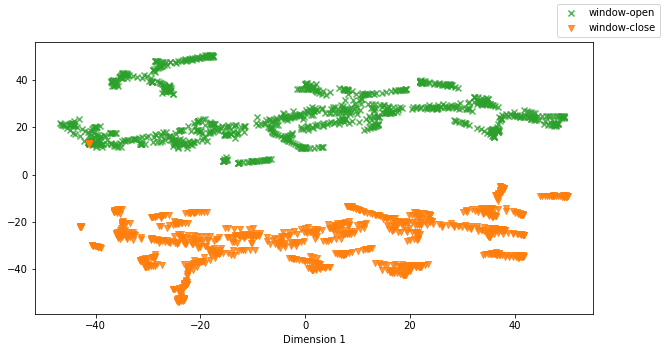
\includegraphics[width=0.9\linewidth]{\FigsDir/EmbeddingSpaceVisualization.png}
  \caption{Visualization of clustering results on task embedding vectors $z^t_S$ and $z^t_T$. Different colors mark different tasks.\label{ch:DTAIL:fig:TSNE}}
\end{figure}


Although the novel idea of applying repetition learning and encoding the task knowledge into a task embedding has significantly improved the adapted agent on both tasks,
there is still one limitation.
As shown in Figure \ref{ch:DTAIL:fig:LearningExperience},
ideally,
the adapted agent should be able to perform both source and target tasks better over time and eventually surpass its performance on the source task before being adapted.
However,
as shown in the experimental results,
there was an amount of deterioration in the source task's performance,
thus,
the proposed method is still limited compared to human learning ability.
Overcoming this problem can be served as a key step toward building a continual learning agent, where the agent can learn and adapt to not only one but multiple target tasks.
In future work,
this will be the main focus of the authors in order to provide a general-purpose agent that can become a better learner over time,
i.e., learning new tasks better and faster,
and performing better on previously learned tasks.
